%----------------------------------------------------------------------------------------
%	PACKAGES AND THEMES
%----------------------------------------------------------------------------------------
\documentclass[aspectratio=169,xcolor=dvipsnames]{beamer}
\usetheme{SimplePlus}

\usepackage{hyperref}
\usepackage{graphicx} % Allows including images
\usepackage{booktabs} % Allows the use of \toprule, \midrule and \bottomrule in tables
\usepackage{fontawesome}
\usepackage{multicol}
%----------------------------------------------------------------------------------------
%	TITLE PAGE
%----------------------------------------------------------------------------------------

\title[Advanced deep neural networks for MRI image reconstruction]{Advanced deep neural networks for MRI image reconstruction from highly undersampled data in challenging acquisition settings
} % The short title appears at the bottom of every slide, the full title is only on the title page
\subtitle{PhD defense}

\author[Zaccharie] {Zaccharie Ramzi}

\institute[Inria-CEA] % Your institution as it will appear on the bottom of every slide, may be shorthand to save space
{
    Parietal team, Inria Saclay \\
    NeuroSpin and Cosmostat, CEA Saclay
}
\date{18th February 2022} % Date, can be changed to a custom date


\setbeamerfont{subsection in toc}{size=\small}
\setbeamerfont{section in toc}{size=\large}


%----------------------------------------------------------------------------------------
%	PRESENTATION SLIDES
%----------------------------------------------------------------------------------------

\begin{document}

\begin{frame}
    % Print the title page as the first slide
    \titlepage
\end{frame}

% Introduction: the problem at hand
% Introduction: physics of MRI
% Acceleration: classics
% Acceleration: CS
% Deep Learning
% Application of DL to MRI: model agnostic, single domain and unrolled networks
% Clinical applicability
% Going further !
% CCL
{
\usebackgroundtemplate{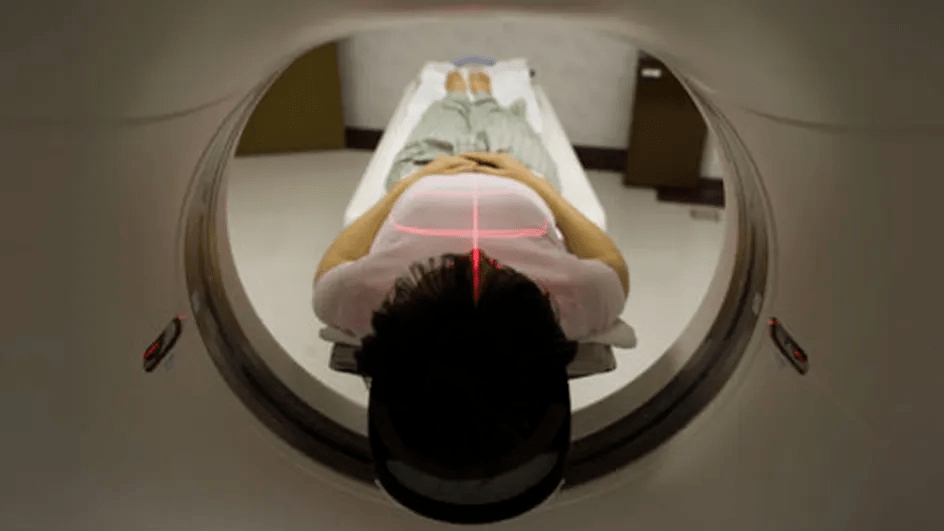
\includegraphics[width=\paperwidth]{Figures/inside_mri.png}}
\begin{frame}[plain]
    % I would like to have the picture of inside the MRI
    % and pass the sound of an MRI scan
    %  \href{run:sons/extract.mp3}{\beamerbutton{écouter}} (https://texnique.fr/osqa/questions/2988/du-son-dans-beamer)
    % https://www.francetvinfo.fr/sante/malgre-l-augmentation-des-besoins-medicaux-le-deficit-en-france-d-appareils-irm-se-fait-de-plus-en-plus-sentir_220301.html
    \href{run:Sounds/mri_sounds.mp3}{\faPlayCircle}
\end{frame}
}

% link between the 2: this is the sound you hear when undergoing an MRI
% now imagine that you will on average hear this during x minutes
% MRI scanners being slow not only generate discomfort but have other impacts on their efficiency...
\begin{frame}{MRI is slow}
    Typical MRI~(Magnetic Resonance Imaging) scan duration: 15 minutes (up to 90 minutes).
    Hence:
    \begin{itemize}
        \item discomfort \& accessibility issues;
        \item reduced patient throughput;
        \item increased motion.
    \end{itemize}
    % give typical duration (compare to CT)
    % give associated problems
\end{frame}

\begin{frame}{Our objective: accelerate MRI scans}
    % give TOC
    \begin{multicols}{2}
    \tableofcontents
    \end{multicols}
\end{frame}

\section{Introduction to MRI}
\subsection{Importance of MRI}
\begin{frame}{Importance of MRI - 1}
    % how many MRI scans / scanners
    % how likely is it that you will get an MRI in your life
\end{frame}

% There is a reason for that: MRI can help diagnose many different conditions
\begin{frame}{Importance of MRI - 2}
    % list of conditions
\end{frame}

\subsection{Physics of MRI}
% MRI is so popular why isnt it solved already ?
\begin{frame}{Physics of MRI - 1}
    % at its core MRI relies on the MR phenomenon
    % in short: a spin is aligned with the magnetic field, when an RF pulse is sent, it tips the spin in the orthogonal plane before the spin realigns with the magnetic field sending another RF pulse
    % video of e-MRI
\end{frame}

\begin{frame}{Physics of MRI - 2}
    % Because all spins get excited, we get a global RF pulse that is the weighted sum of the contribution of all spins' relaxation RF pulses: global information
    % We can obtain "multiple global information", by changing a bit the magnetic field spatially using gradients
    % Signal equation
\end{frame}

\begin{frame}{Physics of MRI - 3}
    % Signal equation => k-space
    % We are sampling in the Fourier space of the anatomical image
\end{frame}

\begin{frame}{Physics of MRI - 4}
    % Let's not forget our initial goal here: we want to understand why MRI is slow
    % The relaxation is slow !
\end{frame}

\subsection{Acceleration in MRI}
\begin{frame}{Where is there room for acceleration?}
    % Explain the concept of redundancy
    % first example: partial Fourier => give limits
\end{frame}

\begin{frame}{Parallel imaging}
    % "forging" the redundancy
    % GRAPPA + SENSE examples
\end{frame}

\begin{frame}{Limits of Parallel Imaging}
    % Max AF
\end{frame}

\section{Compressed Sensing}
\begin{frame}{Structure and redundancy}
    % give a sense of what structure is and how it relates to redundancy
\end{frame}

\subsection{Linear Inverse Problems}
\begin{frame}{Linear Inverse Problems}
    % introduce linear inverse problems
\end{frame}

\begin{frame}{Recovery guarantees}
    % explain the concept of sparsity and its link to recovery guarantees
\end{frame}

\begin{frame}{Application to MRI}

\end{frame}

\subsection{Recovery Algorithms}
\begin{frame}{Relaxation}

\end{frame}

\begin{frame}{ISTA}

\end{frame}

\begin{frame}{Dictionary Learning}

\end{frame}


\begin{frame}{Limitations of classical recovery algorithms}
    % give max AF
    % also give a sense of the limitations in compute and in prior learning
\end{frame}

\section{Deep Learning}

\subsection{The power of Deep Learning}
\begin{frame}{The power of Deep Learning}
    % we want to learn a complicated function that tells us whether an image is an MR image
    % similarly deep learning has been able to build functions that tell whether an image is that of a dog or a cat
    % universal approx
\end{frame}

\begin{frame}{Formalism - 1}
    % supervised learning objective function
\end{frame}

\begin{frame}{Formalism - 2}
    % Stochastic Gradient descent and chain rule
\end{frame}

\subsection{Requirements for Deep Learning}
\begin{frame}{Requirements for Deep Learning}
    % Great that I can do that, but does it take ?
    % Data, compute + memory, framework
    % accept that it's "black-box"
\end{frame}

\begin{frame}{Building the network}
    % give classical functions
\end{frame}

\addtocontents{toc}{\newpage}

\section{Deep Learning for MRI}
\subsection{Simple models}
\begin{frame}{Model agnostic learning}
    % reframing the problem as supervised learning
    % no knowledge of the physics imposed in the model
\end{frame}

\begin{frame}{Single domain learning}
    % Use the backward operator as a basis for the restoration model
\end{frame}

\subsection{Unrolled models}
\begin{frame}{Unrolled models - 1}
    % recovery algorithm and corresponding computation graph
    % show on second slice unrolled computation graph
\end{frame}

\begin{frame}{Unrolled models - 2}
    % move from fixed prior to learned one
\end{frame}

\begin{frame}{Unrolled models - 3}
    % first benchmark: different unrolling strategies give different results

\end{frame}

\subsection{New unrolled models}
\begin{frame}{XPDNet}
    % talk about XPDNet archi
\end{frame}

\begin{frame}{fastMRI challenge}
    % mention fastMRI challenge results
\end{frame}

\begin{frame}{NC-PDNet - 1}
    % explain NC-PDNet and density compensation
\end{frame}

\begin{frame}{NC-PDNet - 2}
    % give results
\end{frame}

\begin{frame}{Recap}
    % cool: we are starting to have good results, let's not forget the end goal
    % use this in a scanner so that the MRI exam is faster
    % how will this technique fare in the clinical setting ?
\end{frame}

\section{Clinical applicability}
\subsection{Learnlets}
\begin{frame}{Learnlets - 1}
    % explain that robustness is a key aspect that we have with wavelets
\end{frame}

\begin{frame}{Learnlets - 2}
    % show the Learnlets model
\end{frame}

\begin{frame}{Learnlets - 3}
    % Learnlets results
\end{frame}

\subsection{Denoising Score Matching}
\begin{frame}{Denoising Score Matching - 1}
    % explain what UQ might be used for
\end{frame}

\begin{frame}{Denoising Score Matching - 2}
    % give method of DSM
\end{frame}

\begin{frame}{Denoising Score Matching - 3}
    % give results
\end{frame}

\subsection{Comparison with GRAPPA}
\begin{frame}{Prospective comparison with GRAPPA}
    % show big brain results
    % explain why it's robustness test already
\end{frame}

\begin{frame}{Recap}
    % we have seen how to adapt to clinical setting and answered the question of prospective reconstruction
    % robust : learnlets
    % UQ: DSM
    % propsective: check
\end{frame}

\section{Going even deeper}
\subsection{Implicit models}

\begin{frame}{Why should we go deeper?}
    % with deeper models, comes better performance
    % figure of Pezzotti et al.
\end{frame}

\begin{frame}{Can we go deeper?}
    % in the current state not: activations + constrained memory
\end{frame}

\begin{frame}{The modeling solutions}
    % gradient checkpointing
    % Invertible networks
    % Implicit models
\end{frame}

\begin{frame}{Deep Equilibrium networks}
    % give equation and how to compute the gradient with IFT
\end{frame}

\subsection{SHINE}
\begin{frame}{The limits of DEQs}
    % they are slow to train
\end{frame}

\begin{frame}{Why are DEQs slow?}
    % bc of Jacobian inversion
\end{frame}

\begin{frame}{Can we avoid the Jacobian inversion?}
    % yes: reuse a by-product of the forward pass, share the inverse estimate
\end{frame}

\begin{frame}{Application to Hyperparameter optimization}
    % it's also a bilevel prob
\end{frame}

\begin{frame}{Results on DEQs}

\end{frame}

\section{Conclusion \& Future works}

\begin{frame}{Conclusion}
    % what have we seen so far in the journey?
\end{frame}

\begin{frame}{Future works}
    % DEQs for MRI recon
    % More operator correction
    % Trajectory learning
\end{frame}
%----------------------------------------------------------------------------------------

\end{document}